%\documentclass[jou]{apa6}
\documentclass[11pt]{article}
\usepackage{ucs}
\usepackage[utf8x]{inputenc}
\usepackage{changepage}
\usepackage{graphicx}
\usepackage{amsmath}
\usepackage{gensymb}
\usepackage{amssymb}
\usepackage{enumerate}
\usepackage{tabularx}
\usepackage{lipsum}
\usepackage{hyperref}
\usepackage{fancyvrb}
\usepackage{mathtools}
\usepackage{color}

\oddsidemargin 0.0in
\evensidemargin 0.0in
\textwidth 6.27in
\headheight 1.0in
\topmargin -0.1in
\headheight 0.0in
\headsep 0.0in
\textheight 9.0in

\usepackage{xcolor}


\setlength{\parindent}{0pt}
\setlength{\columnsep}{1cm}

\newenvironment{myenv}{\begin{adjustwidth}{0.4in}{0.4in}}{\end{adjustwidth}}
\renewcommand{\abstractname}{Anotācija}
\renewcommand\refname{Atsauces}



\newcounter{alphnum}
\newenvironment{alphlist}{\begin{list}{(\Alph{alphnum})}{\usecounter{alphnum}\setlength{\leftmargin}{2.5em}} \rm}{\end{list}}


%16.3-6

\makeatletter
\let\saved@bibitem\@bibitem
\makeatother

\usepackage{bibentry}
%\usepackage{hyperref}


%\title{Homework 1: Grading Criteria}
%\author{Kalvis}
%\affiliation{RBS}



\begin{document}
\thispagestyle{empty}

\twocolumn


\begin{center}
{\Large Assignment 3, 2020-10-01},\\
{\em Estimated time: 12 minutes}
\end{center}

\vspace{10pt}
{\bf Question (Vector Operations)}\\ The data structure {\tt std::vector} 
supports operation {\tt push\textunderscore{}back(elt)} (append {\tt elt} 
to the end of the vector), {\tt pop\textunderscore{}back()} (delete the last element), 
and {\tt at(i)} (return the element at the $i$-th position of the vector. 


\vspace{10pt}
Source file {\bf File1.cpp}:
{\footnotesize
\begin{center}
\begin{minipage}{.85\columnwidth}
\begin{Verbatim}[frame=single,numbers=left]
#include <iostream>
#include <vector>

using namespace std;
void VECTOR_PRINT(vector<int> v) {
  vector<int>::iterator i;
  for (i=v.begin(); i!=v.end(); ++i)
    cout << (*i) << ".";
  cout << endl;
}

int main() {
  // 3 digits from your student ID
  int a, b, c; 
  cin >> a >> b >> c;
  vector<int> vv;
  vv.push_back(9);
  vv.push_back(7);
  vv.push_back(c);
  VECTOR_PRINT(vv);
  vv.push_back(vv.at(2));
  vv.push_back(vv.at(1));
  VECTOR_PRINT(vv);
  vv.pop_back();
  vv.push_back(b);
  vv.push_back(a);
  vv.pop_back();
  VECTOR_PRINT(vv);
  return 0;
}
\end{Verbatim}
\end{minipage}
\end{center}
}


Assume that somebody runs this program, and 
uses numbers {\tt a, b, c} 
that are the last three digits from your Student ID number. 
For example, this Student ID:

\vspace{2pt}
{\LARGE 191RDB876}\\
has {\tt a=8}, {\tt b=7}, {\tt c=6}.

\vspace{10pt}
Function {\tt VECTOR\textunderscore{}PRINT(...)} is called three times in 
this code (Lines 20, 23 and 28). 
Draw the state of the {\tt vector} data structure at these three moments in time.

{\footnotesize
\begin{Verbatim}[frame=single,numbers=left]
vector<int> vv;
vv.push_back(101);
vv.push_back(102);
vv.push_back(103);
\end{Verbatim}
}


For example, the above code fragment would create vector 
state shown in the Figure below:

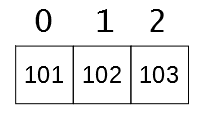
\includegraphics[width=0.8in]{assignment03-stl/assignment03-vector-state.png}


\vspace{10pt}
{\bf (A) The state of vector {\tt vv} on Line 20:}

\vspace{50pt}
{\bf (B) The state of vector {\tt vv} on on Line 23:}

\vspace{50pt}
{\bf (C) The state of vector {\tt vv} on on Line 28:}



\end{document}

